\documentclass[article]{beamer}
\usetheme{Warsaw}
\setbeamertemplate{footline}[frame number]

\usefonttheme[]{serif}
\usepackage{amsmath, latexsym, color, graphicx, amssymb, bm, here}
\usepackage{epsf, epsfig, pifont,tikz,subfigure}
\usepackage{graphics, calrsfs}
\usepackage{times}
\usepackage{fancybox,calc}
\usepackage{palatino,mathpazo}
\usepackage{amsfonts}
\usepackage{sidecap}
\usepackage{listings}
\usepackage{hyperref}

\title{Dynamic Programming}
\author{David Jacobo \\ \href{mailto:jguillen@cimat.mx}{jguillen@cimat.mx}}
\date{\scriptsize{\today}}

\AtBeginSection[]
{
  \begin{frame}{Outline}
    \tableofcontents[currentsection]
  \end{frame}
}

\begin{document}

%%%%%%%%%%%%%%%%%%%%%%%%%%%%%%
\maketitle

%%%%%%%%%%%%%%%%%%%%%%%%%%%%%%
\begin{frame}
\begin{block}{Dynamic Programming (DP):}
	Also called \textbf{'memoization'} is a paradigm focused on solving \textbf{optimization 
	problems}. For a problem to be solved with DP, it must exhibit an \textbf{optimal substructure and
	overlapping sub-problems}.
	
	\vspace{8mm}
	
	A critical part on designing DP solutions boils down to recognizing/defining the 
	required \textbf{state and transitions}. There are two typical ways to express a DP solution: \textbf{bottom up and top down}.
\end{block}
\end{frame}

%%%%%%%%%%%%%%%%%%%%%%%%%%%%%%

\section{Basics}

\subsection{Motivation}
\begin{frame}
	\frametitle{Fibonacci series: Recurrence formula}
	\begin{equation}
		FIB(N)=\begin{cases}
		1, & \text{when } N \leq 1 \\
		FIB(N-2) + FIB(N-1), & \text{otherwise.}
		\end{cases}
	\end{equation}
	
	\vspace{8mm}
	
	For some instances we actually know the solution, those are the \textbf{base cases}.
\end{frame}

\begin{frame}
	\frametitle{Fibonacci series: Recurrence tree}
	\begin{center}
		\includegraphics[scale=0.7]{./figures/fib.eps}
	\end{center}
\end{frame}

\subsection{Properties}
\begin{frame}
	\frametitle{Optimal substructure}
	Refers to the fact that you need to know the \textbf{optimal solution for smaller instances} in order to expand your solution to the required size.
	
	\vspace{8mm}
	
	\begin{center}
		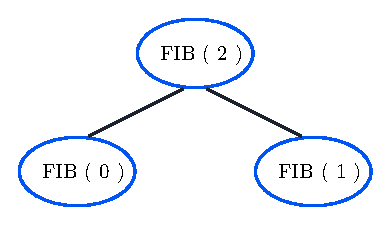
\includegraphics[scale=0.8]{./figures/zoom.eps}
	\end{center}
\end{frame}

\begin{frame}
	\frametitle{Overlapping sub-problems}
	Whenever you are calling the exact instance of the problem 2 or more times it's clear than an overlap exists.
	
	\vspace{1mm}
	
	\begin{center}
		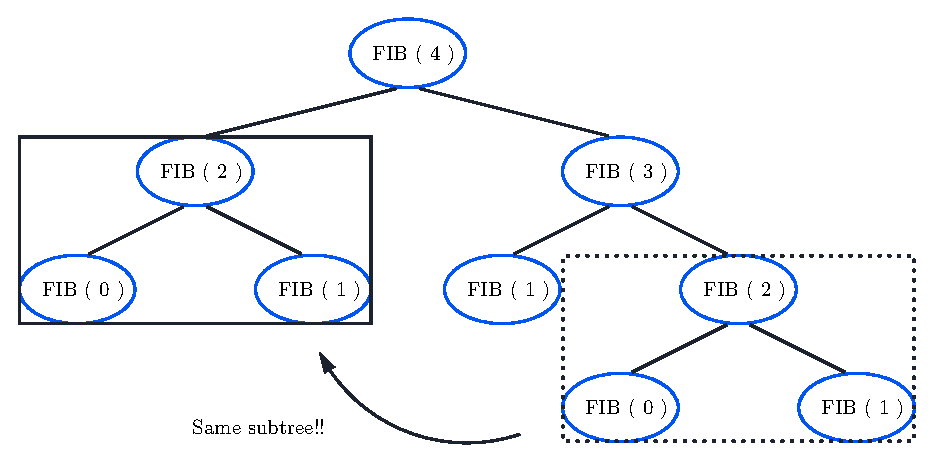
\includegraphics[scale=0.6]{./figures/overlaps.eps}
	\end{center}	
\end{frame}

\begin{frame}
	\frametitle{State}
		A state is the list of parameters which represent each sub-problem in a unique way.
		
		\vspace{8mm}
		
		For our example, an integer suffices to represent each state:
		\begin{center}
			\includegraphics[scale=0.9]{./figures/fib_series.eps}
		\end{center}
		
\end{frame}

\begin{frame}
	\frametitle{Transition}
		A transition defines if you can directly pass from an state A, to an state B.
		
		\vspace{8mm}
		
		In this example a line represent the different transitions available, all of them relates N to N-1 and N-2, just like in the formula.
		\begin{center}
			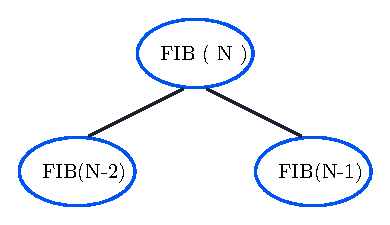
\includegraphics[scale=0.9]{./figures/transitions.eps}
		\end{center}
\end{frame}

\section{Design and coding styles}

\subsection{Bottom up}
\begin{frame}[fragile]
	\frametitle{Bottom up}
	This variant solves and store the solutions for \textbf{all the smaller instances} before solving the bigger instance (which is the one that matters for us).
	
	\vspace{2mm}
	\footnotesize{
	\begin{lstlisting}
 0      int state[A_LOT];
 1      state[0] = state[1] = 1;	
 2	
 3      int fib(int N){
 4          for(int i=2;i<= N;++i)
 5              state[i] = state[i-1] + state[i-2]; 
 6 
 7          return state[N];
 8      }
	\end{lstlisting}
	}
\end{frame}

\subsection{Top down}
\begin{frame}[fragile]
	\frametitle{Top down}
	The top down approach relies in calling only the instances which are really needed for the given problem.
	
	\vspace{2mm}
	\footnotesize{
	\begin{lstlisting}
 0      int state[A_LOT];
 1      memset(state, NOT_CALC, sizeof(state));
 2      state[0] = state[1] = 1;
 3	
 4      int fib(int N){
 5          if(state[N]!=NOT_CALC)    return state[N];
 6			
 7          return state[N] = (fib(N-1) + fib(N-2));
 8      }
	\end{lstlisting}
	}
\end{frame}

\subsection{Fight!}
\begin{frame}
	\frametitle{So, which one is better?}
	Remember that both are based on the same recurrence formula, thus they are equaly correct.
\end{frame}

\section{Algorithm analysis}

\subsection{Time complexity}
\begin{frame}
	\frametitle{Time complexity}
	Time complexity refers to the amount of time it will take to your algorithm to finish in terms of a given input. 
	
	\vspace{8mm}	
	
	\begin{center}
	\textbf{O(M * S)}
	\end{center}
	
	\vspace{8mm}
	
	where: M stands for the total different states and S stands for the complexity of calculating each state.
\end{frame}

\subsection{Space complexity}
\begin{frame}
	\frametitle{Space complexity}
	The space complexity refers to the amount of memory necessary to store all the answers, so it basically express how many states your problem has.
	
	\vspace{8mm}
	
	\begin{center}
	\textbf{O(M)}
	\end{center}
	
	\vspace{8mm}
	
	where M stands for the total different states.
\end{frame}

\section{Classic problems}
\begin{frame}
	Again, the core of DP is finding the \textbf{optimal solution} for a problem, ranging from strings processing to robotics!

	\vspace{8mm}

	\begin{itemize}
		\item Longest Common Subsequence
		\item Edit Distance
		\item Single Source Shortest Path
		\item Coin Change
		\item Knapsack
		\item Floyd-Warshall
	\end{itemize}
\end{frame}

\section{Pro-tips}
\begin{frame}
	\frametitle{Pro-tips}
	\begin{itemize}
		\item Study the theory.
		\item Write solutions for the classic problems.
		\item Compare bottom-up vs top-down.
	\end{itemize}
	
	\vspace{5mm}
	
	It is also worthy to explore the \textbf{sliding window} trick in order to save memory, or selecting a \textbf{different data structure} for saving the intermediate states specially when using the top-down approach. \textbf{DP is a trade-off between space and time!}
\end{frame}

%%%%%%%%%%%%%%%%%%%%%%%%%%%%%%
\begin{frame}[plain]
\frametitle{}
\begin{center}
\Huge{\color{blue}{Q \& A}}
\end{center}
\end{frame}

%%%%%%%%%%%%%%%%%%%%%%%%%%%%%%%%
\begin{frame}[plain]
	\textbf{References}
	\begin{itemize}
		\item \href{https://sites.google.com/site/stevenhalim/}{Competitive Programming site}
		\item \href{https://github.com/davidjacobo/algorists/}{Algorists' repository}
	\end{itemize}
\end{frame}
\end{document}